


%.....................................
\subsubsection{Gravity meters}


include here pic of Vening Meinesz

\begin{center}
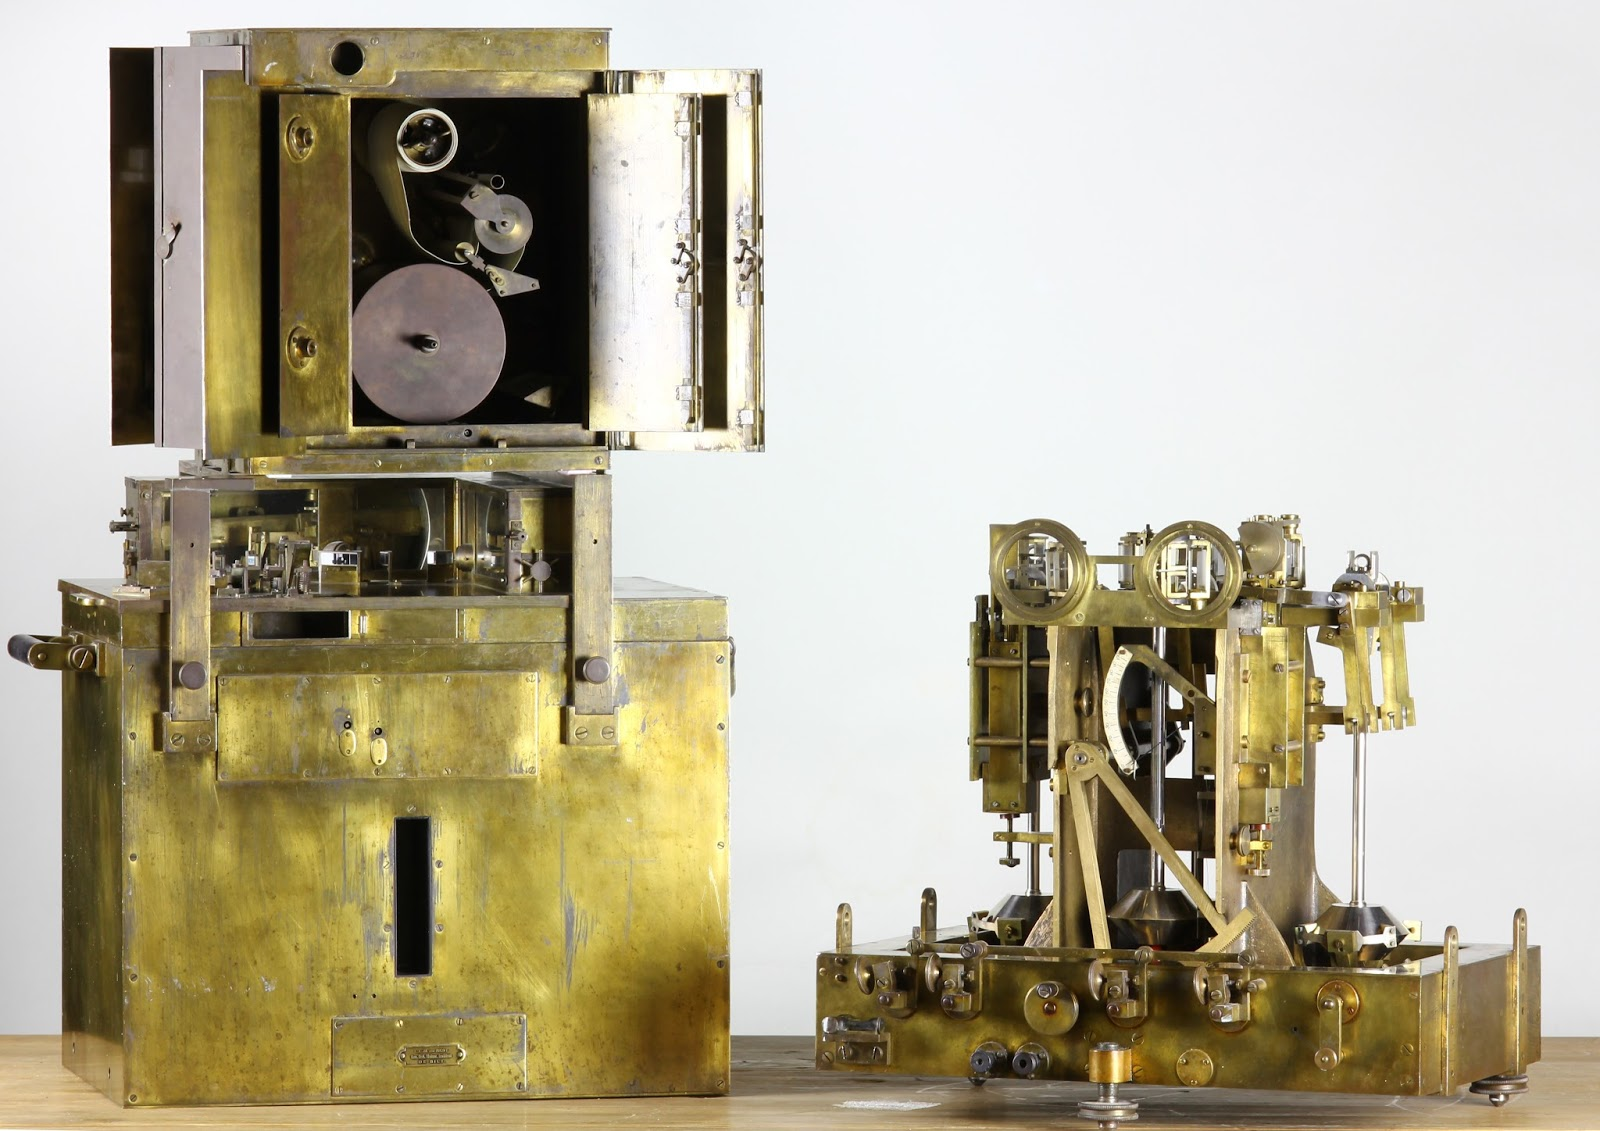
\includegraphics[width=10cm]{images/gravity/Gouden_kalf}\\
{\captionfont 
Taken from 
website\footnote{\url{http://deepearthscience.blogspot.com/2016/06/the-gravimeter-of-professor-vening.html}}.
The pendulum apparatus of Vening Meinesz, also known as "Het Gouden Kalf" (the Golden Calf). Positioned on the left side is the protective casing with the recording instrument on top. On the right side is the pendulum apparatus with the three pendulums at the back. }
\end{center}


\paragraph{Absolute gravity measurements}

After a time $t$ an object has fallen by a distance $x$ in a gravity field $g$
with $x=gt^2/2$ so that $g=2x/t^2$.

\begin{center}
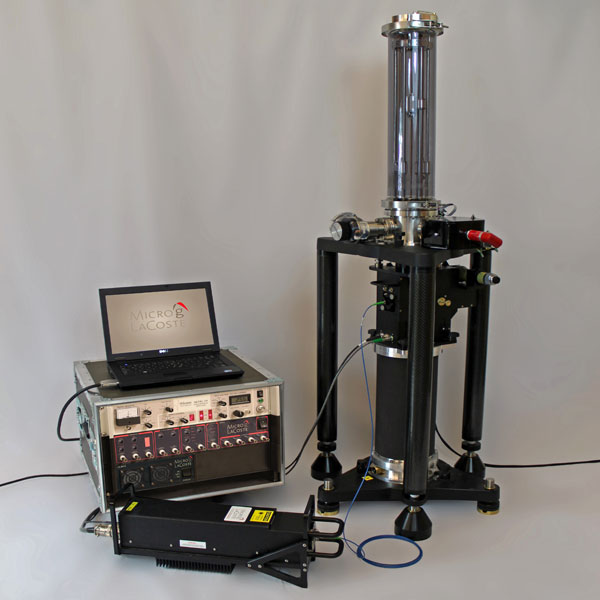
\includegraphics[width=6cm]{images/gravity/fg5}\\
{\captionfont by Micro-g LaCoste. 
The FG5\footnote{\url{http://microglacoste.com/product/fg5-x-absolute-gravimeter/}}
 operates by using a free-fall method. An object is dropped inside a vacuum 
chamber and its position is monitored very accurately using a laser interferometer. 
Dropping chamber of 33cm. Accuracy of approx. $2\mu$Gal.}
\end{center}



%.....................................
\subsubsection{Planes}

\begin{center}
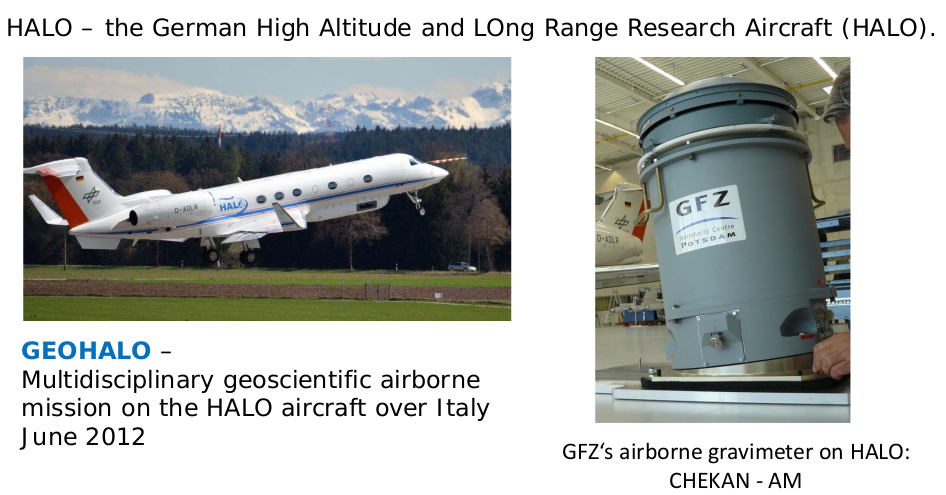
\includegraphics[width=12cm]{images/gravity/halo}
\end{center}





%.....................................
\subsubsection{Satellites}

\paragraph{GRACE}

Note that GRACE consists of two satellites
which are in a low orbit and the distance between them
is accurately measured. Changes in this
separation are caused by increases and decreases
in gravity.

\begin{center}
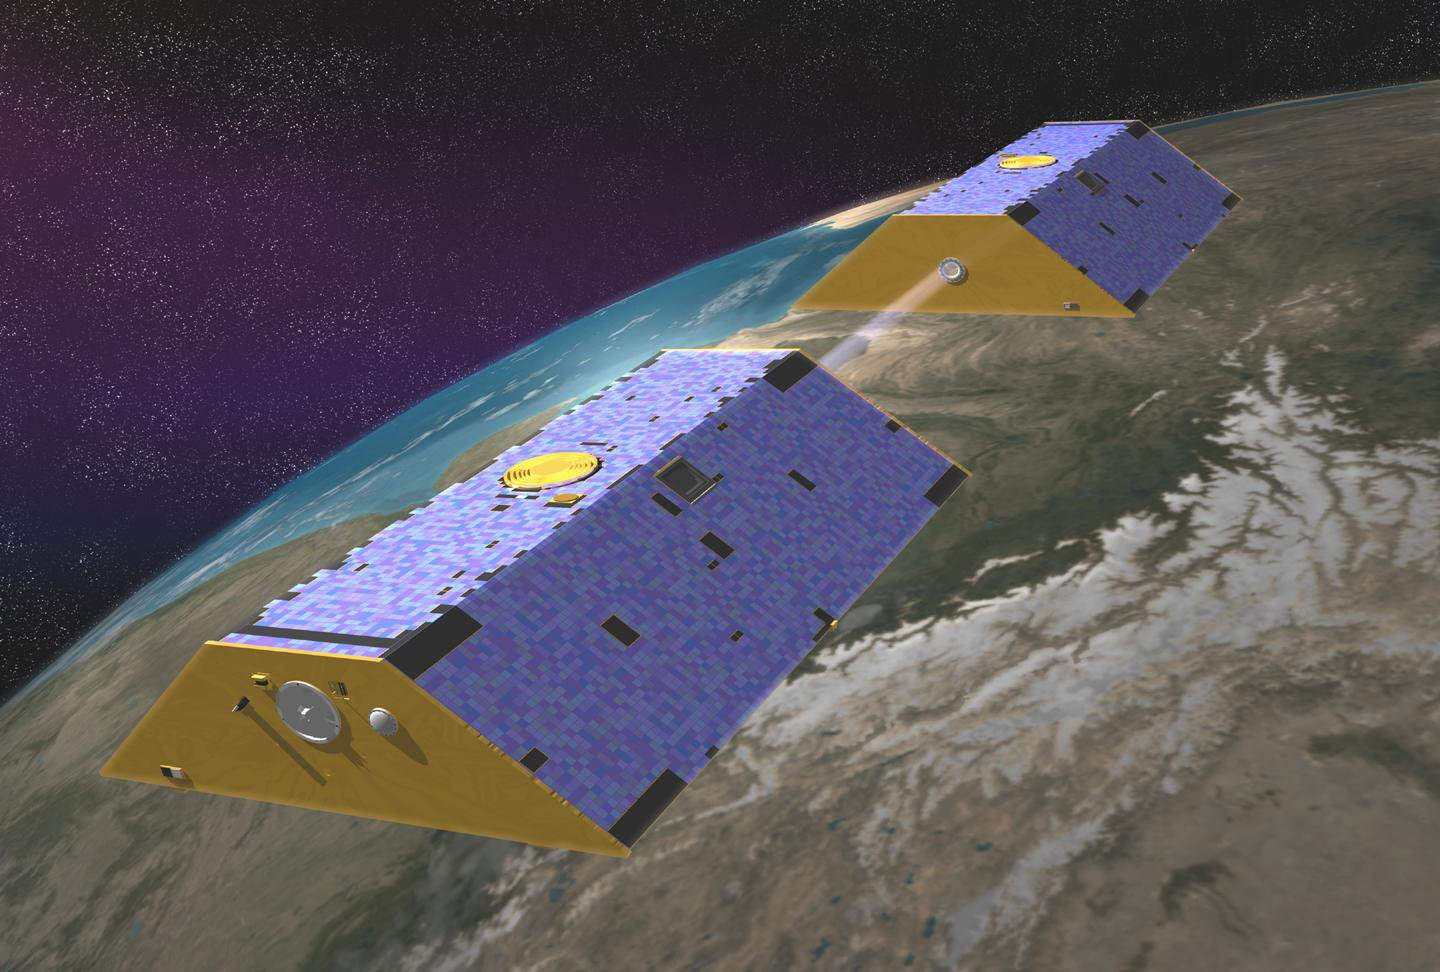
\includegraphics[width=8cm]{images/gravity/GRACE_artist_concept}\\
{\captionfont \url{https://upload.wikimedia.org/wikipedia/commons/e/e6/GRACE_artist_concept.jpg}}
\end{center}


Examples of applications using GRACE data:
\begin{itemize}
\item Inference of mantle viscosity from GRACE and relative sea level data \cite{pazw07}
\item Exploring the uncertainty in GRACE estimates of the mass
redistributions at the Earth surface: implications for the global water
and sea level budgets \cite{blml18}
\end{itemize}




\paragraph{GOCE}

Gravity Field and Steady-State Ocean Circulation Explorer (GOCE) was the first of ESA's 
Living Planet Programme satellites intended to map in unprecedented detail the Earth's gravity field
with a spatial resolution up to 80 km.
The spacecraft's primary instrumentation was a highly sensitive gravity gradiometer consisting of 
three pairs of accelerometers which measured gravitational gradients along three orthogonal axes.



\begin{center}
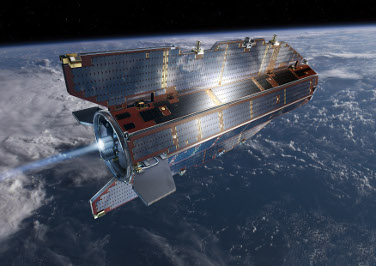
\includegraphics[width=7cm]{images/gravity/goce}
\end{center}

Examples of applications using GOCE data:
\begin{itemize}
\item GOCE gravitational gradients along the orbit \cite{boff11}
\item Moho Estimation Using GOCE Data: A Numerical Simulation \cite{resa12}
\item Global Moho from the combination of the CRUST2.0 model and GOCE data \cite{ress13}
\item Advancements in satellite gravity gradient data for crustal studies \cite{ebbf13}
\item Sensitivity of GOCE Gravity Gradients to Crustal Thickness and Density Variations: Case Study
for the Northeast Atlantic Region \cite{ebbf14}
\item Mapping the mass distribution of Earth’s mantle
using satellite-derived gravity gradients \cite{papg14}
\item GOCE gravity gradient data for lithospheric modeling \cite{boem15}
\item Exploration of tectonic structures with GOCE in Africa and across-continents \cite{brai15}
\item GEMMA: An Earth crustal model based on GOCE satellite data \cite{resa15}
\item GOCE data, models, and applications: A review \cite{vapb15}
\item Geological units and Moho depth determination in the Western Balkans exploiting GOCE data \cite{samp15}
\item The combined inversion of seismological and GOCE gravity data: New
insights into the current state of the Pacific lithosphere and upper mantle \cite{togr17}
\end{itemize}

